\documentclass[]{beamer}
%%\documentclass[notes]{beamer}
\usepackage{etex}

%% Default will be false for \handouts; it can be set to true within
%% the Makefile.

\newcommand{\adv}{{\tiny (Advanced)}}

\usepackage{showexpl,xspace}
\usepackage{ifthen}
\usepackage{amsmath}

\providecommand*{\handouts}{false}
\ifthenelse{\equal{\handouts}{true}}
{\usepackage{pgfpages}
  \pgfpagesuselayout{4 on 1}[a4paper,landscape]}
{}
%% Handling handouts: end %%%%%%%%%%%%%%%%%%%%%%%%%%%%%%%%%%%%%%%%%%%%%%





%% \newcommand{\pauseb}{}

%% fragwidth will measure the width of the text, and then we use
%% it for the width of the textblock.
\newdimen{\fragwidth}

\newcommand{\mybottomleft}[1]{
\settowidth{\fragwidth}{#1}
\begin{textblock*}{\fragwidth}[0,0](2mm,90mm)  %% {width}(horiz, vert)
  #1
\end{textblock*}
}

\newcommand{\mybottomright}[1]{
\settowidth{\fragwidth}{#1}
\begin{textblock*}{\fragwidth}[1,0](126mm,90mm)  %% {width}(horiz, vert)
  #1
\end{textblock*}
}

\usepackage{graphicx}

\def\0{\hbox{\phantom{\footnotesize\rm 0}}}

%% Seek help from beamer crowd about this?
\makeatletter
\def\DIfF^#1{%
  \mathop{\mathrm{\mathstrut \text{d}}}%
  \nolimits^{#1}\gobblespace}
\makeatother

%% This snippet is from the TeX faq and allows us to use \maxwidth
%% for the max size of an image.
\makeatletter
\def\maxwidth{%
  \ifdim\Gin@nat@width>\linewidth
  \linewidth
  \else
  \Gin@nat@width
  \fi
}
\makeatother
\usepackage[overlay]{textpos}

\mode<presentation>
{
  \setbeamersize{text margin left=0.25cm}
  \setbeamersize{text margin right=0.25cm}

  \beamertemplatedotitem

  \beamertemplateheadempty %% Remove headline (at top of frame)
  %% \beamertemplatefootempty %% Remove headline (at top of frame)
  %% \beamertemplatefootpagenumber %% page number only in footer.
  %% Remove navigation icons.
  \setbeamertemplate{navigation symbols}{}

  %% Show start of every lecture. Not available in article.
  \AtBeginLecture{\frame{\Large Lecture \insertlecture}}
}




\title{\LaTeX\ 101}
\author{Stephen J. Eglen}


\institute{Cambridge Computational Biology Institute\\
  Department of Applied Mathematics and Theoretical Physics\\
  University of Cambridge\\
  \url{http://www.damtp.cam.ac.uk/user/eglen/}
}

\date{October 2014}

\begin{document}

\begin{frame}
  \titlepage
\end{frame}

\begin{frame}
  \frametitle{What is \LaTeX?}
  \begin{itemize}
  \item Typesetting, not WYSIWYG.
  \item Given a source file (file.tex) you \textbf{compile} your document (file.pdf).
  \item Heavily used by mathematicians/scientists/publishers for
    formatting papers/books.
  \item Logical markup of your document (like HTML) rather than
    specifying exactly how you want it look.
  \item Use Word (or document of your choice) if you want to.

  \item You can typeset music, chessboards, wiring diagrams, ...

  \item These slides are written in matex using the ``beamer'' package.

  \end{itemize}
\end{frame}


\begin{frame}[fragile]
  \frametitle{``Hello world'' example}

\section*{hi there}
  \begin{LTXexample}[pos=b,rframe={}]
  \documentclass{article}
  \begin{document}
    Hello world.  Welcome to \LaTeX.
  \end{document}
\end{LTXexample}
%% Complicated begin/end documents don't work in beamer.
%%http://tex.stackexchange.com/questions/6006/how-to-use-showexpl-with-an-external-class
\end{frame}


\begin{frame}[fragile]
  \frametitle{Another example}

Taken from \url{showexpl-test.tex}
\begin{LTXexample}[pos=b,wide,width=.65,preset=\LARGE,rframe={}]
\documentclass[a4paper,twoside]{article}
\begin{document}
  \begin{equation}
    \sigma(t)=\frac{1}{\sqrt{2\pi}}
    \int^t_0 e^{-x^2/2} dx 
  \end{equation}
\end{document}
\end{LTXexample}

\end{frame}

\begin{frame}
  \frametitle{Getting started}

  Install texstudio or some other latex.  Lots of editors/GUIs
  available.

  \url{http://www.lyx.org} = latex engine + WYSIWG interface.
  
  texstudio handles all the compilation steps for you and provides
  easy way of forward/inverse searching (Ctrl+ left mouse button).
  
\end{frame}

\begin{frame}
  \frametitle{Welcome to the 21st century}

  Many matex guides describe how you can create .dvi files and .ps
  (postscript) files.  

  Ignore that; we typically create .pdf files now, via 'pdflatex'.

  Create your graphs etc in pdf wherever you can, else png/jpg (not
  postscript).

\end{frame}

\begin{frame}[fragile]
  \frametitle{matex syntax - commands}

  \begin{itemize}
  \item matex commands start with backslash and are case-sensitive:

    \begin{LTXexample}[pos=b]
      The \large cat \LARGE sat on \Huge the \normalsize mat
    \end{LTXexample}

    \item Commands can take compulsory {} and optional [] arguments.
      \begin{LTXexample}[pos=b]
        A \rule{10mm}{3mm}  B \rule[-1mm]{10mm}{3mm}  
      \end{LTXexample}
  \end{itemize}
\end{frame}


\begin{frame}[fragile]
  \frametitle{Environments}

An environment is a block of latex code to provide some
functionality.  They can be nested.
\begin{LTXexample}[pos=r]
  \textbf{Top TV programmes}:
  \begin{enumerate}
  \item Homeland
  \item The West Wing
    \begin{itemize}
    \item Series 1
    \item (Not series 3)
    \end{itemize}
  \item 24
  \end{enumerate}
\end{LTXexample}
\end{frame}



\begin{frame}[fragile]
  \frametitle{Typesetting math}

  \begin{enumerate}
  \item matex normally is in tex mode.  You must switch to math mode
    using \$ to get into and out of math.
\begin{LTXexample}[pos=b]
  This equation $x^2 + y^2 = z^2$ is in-line; compare with:
  \begin{eqnarray}
    \label{eq:key}
    I_1 &= \int_0^{2 \pi} \sin (x^2) dx \nonumber \\
    \text{but}\, I_2 &= \int_0^{2 \pi} \cos (x^2) dx \label{key}
  \end{eqnarray}
  The dx in Equation \ref{key} needs fixing later \ldots
\end{LTXexample}
    
  \end{enumerate}
\end{frame}


\begin{frame}
  \frametitle{amsmath -- AMS mathematical facilities for matex}

  \url{http://mirrors.ctan.org/macros/latex/required/amslatex/math/amsldoc.pdf}

  Lots of good examples for formatting maths.  See the examples in:

  \url{http://mirrors.ctan.org/macros/latex/required/amslatex/math/testmath.pdf}

\end{frame}
\begin{frame}
  \frametitle{Universe of mathematics symbols and operators}
\end{frame}

\begin{frame}
  \frametitle{Finding maths operators}

websites to check.  Draw on it.
\end{frame}


\begin{frame}[fragile]
  \frametitle{Defining your own commands}


  \begin{LTXexample}[pos=b]
    \newcommand{\betaIIKO}
    {\ensuremath{\beta\mathit{2}^{-/-}}\xspace}
    The \betaIIKO mouse is widely studied \ldots 
    the \betaIIKO command  is easier for me
    to type than the whole expansion.

    \newcommand{\nnn}[1]{\ensuremath{#1^{#1^{#1}}}}
    Or we can compare \nnn{3} with \nnn{16}.
  \end{LTXexample}

\textit{Typesetting mathematics for science} has many hints for
getting things just write, e.g. the differential operator ``d'' as in
``dx'' and partial, total derivatives:

\url{http://www.tug.org/TUGboat/Articles/tb18-1/tb54becc.pdf}


\end{frame}


\begin{frame}
  \frametitle{Bibliography / citations}

See intro.tex for detailed guide.
zotero/paperpile/mendeley/google scholar all generate good bibtex
entries.

\end{frame}



\begin{frame}[fragile]
  \frametitle{Space}

  \begin{itemize}
  \item Multiple space characters treated as one space.
  \item Blank lines denote paragraph separators.
  \item Non-breaking space \verb+3~mm+ $\Rightarrow$ 3~mm
  \item Small non-breaking space \verb+3\,mm+ $\Rightarrow$ 3\,mm
  \end{itemize}
\end{frame}
\begin{frame}
  \frametitle{Command line material \adv }

  If you run from the command line, you need to follow instructions on
  how often to re-reun matex to resolve references.

  latexmk, texi2pdf help with this problem.

\end{frame}


\begin{frame}[fragile]
  \frametitle{Preamable}

  \begin{enumerate}
  \item Everything before the \verb+begin{document}+ is the preamble.
  \item Use it to set up document, load packages.  My favourite
    packages:


\begin{verbatim}
\usepackage{graphicx}           % Needed for including graphics.
\usepackage{url}                % Facility for activating URLs.
\usepackage[a4paper,margin=2cm]{geometry}
\usepackage{mathpazo}           % of mathptmx
\usepackage{amsmath}            % AMS Maths goodies
\end{verbatim}
  \end{enumerate}
\end{frame}


\begin{frame}
  \frametitle{Your choice of fonts}

  Choose a font that has good support for both math and text modes:

  \begin{enumerate}
  \item Do nothing.  Stick with Donald Knuth's \textit{Computer Modern}.  
  \item I prefer mathpazo (Palatino) or mathptmx (Times).
  \item Explore the free guide \url{http://mirrors.ctan.org/info/Free_Math_Font_Survey/en/survey.html}
  \end{enumerate}
\end{frame}


\begin{frame}
  \frametitle{Floats: tables and figures}

  \begin{itemize}
  \item Floats are objects (tables, figures) that move in your
    document; matex will move them to somewhere it thinks sensible.
  \item If you don't like where it put a float, relax.  You can give
    it hints, but normally it does a good job.
  \item You can then refer to figures/tables by labels.
  \end{itemize}
\end{frame}

\begin{frame}[fragile]
  \frametitle{Tables}

  \begin{LTXexample}[pos=b]
\begin{table}
  \centering
  \begin{tabular}{|l|rr|}  \hline
    year & min temp (C) & max temp (C)\\ \hline
    1970 & -5 & 35\\
    1980 & -3 & 30\\
    1985 & -2 & 32\\ \hline
  \end{tabular}
  \caption{Fictional min/max temperatures.} \label{tab:simple}
\end{table}
  \end{LTXexample}
\end{frame}

\begin{frame}[fragile]
  \frametitle{Figures}

  \begin{LTXexample}
\begin{figure}
  \centering
  \fbox{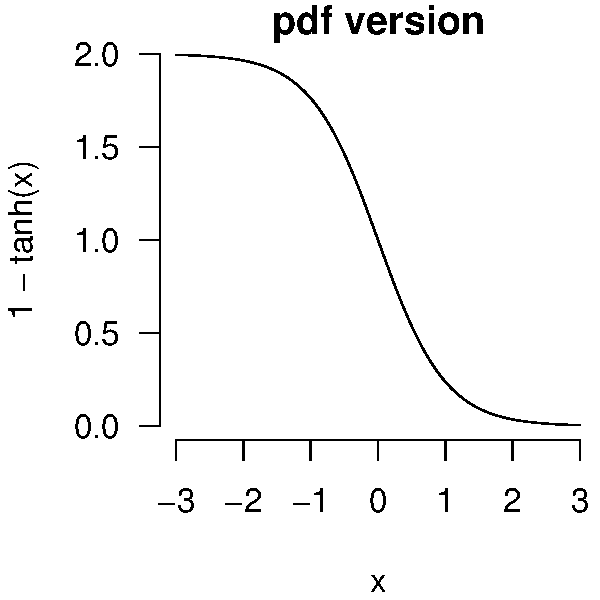
\includegraphics[width=6cm]{sigmoid}}
  \caption{Example of a sigmoidal curve.}
  \label{fig:example}
\end{figure}
  \end{LTXexample}

Looks for file in current directory (or you can keep a path of figures).
\end{frame}


\begin{frame}
  \frametitle{History of matex}
\end{frame}

\begin{frame}
  \frametitle{Advanced topics}

  lualatex is the long-term future.

  Reproducible research documents.
\end{frame}


\begin{frame}[fragile]
  \frametitle{Labels and references}
  \label{labels}
  \begin{enumerate}
  \item For complex documents, rather than writing ``Table 3'', it is
    better to give the Table a label using \verb+\label{results}+, and then refer to that label,
      using e.g. \verb+See Table \ref{results}+.  

      \item You can also refer to figures, equations, sections in a
        similar way.  

        \item To refer to pages you can do:
          \begin{LTXexample}[pos=b]
            This is on page \pageref{labels}.
          \end{LTXexample}
  \end{enumerate}
\end{frame}
\begin{frame}
  \frametitle{Getting help}
  \begin{enumerate}

  \item Work through Lamport's book slowly and surely.
    
  \item Google what you need to.  Often you can find good answers on
    \url{http://tex.stackexchange.com/}

  \item Keep it simple for now!  Focus on the content, not the form.

  \item \textit{The matex companion} lists vast number of packages.
  \end{enumerate}
\end{frame}

\begin{frame}
  \frametitle{TODO}
Draw some equations and it will try to render it in latex or mathml.

http://webdemo.myscript.com/#/demo/equation wolfram thing for text ->
latex

http://mirror.ox.ac.uk/sites/ctan.org/info/symbols/comprehensive/symbols-a4.pdf

http://detexify.kirelabs.org/classify.html

superscripts: can omit braces if superscript is one character: $x^3$
versus $x^{19}$ versus $x^19$.

\end{frame}

\begin{frame}
  \frametitle{End}
\end{frame}

\end{document}

% LocalWords:  Presynaptic heterotypic Homotypic

